\documentclass[a4paper, 12pt, UTF8]{article}

\usepackage[dvipsnames]{xcolor} % Code highlighting color
\usepackage[catalan]{babel} % Language 
\usepackage{indentfirst}
\usepackage{fontspec} 
\usepackage{fullpage}
\usepackage[a4paper, margin=2cm]{geometry} % To change the margins
\usepackage{graphicx} % Insert images
\usepackage[hidelinks]{hyperref} % Links color
\usepackage[final]{pdfpages}
\usepackage{ragged2e}
\usepackage{wrapfig} %To Text wrap
\usepackage{listings} % Add code
\usepackage{verbatim}
\usepackage{nameref}
\usepackage{tikz}
\usepackage{subcaption}
\usepackage{multirow}
\usepackage{colortbl}

\setlength{\parskip}{0.7em}
%\setlength{\parindent}{1cm}
\linespread{1.2}
\setcounter{secnumdepth}{5}

\title{
	\Huge
	\textbf{Pràctica 2} \\ 
	\scshape Sistema Basat en el Coneixement
	}
\author{
	Marc Asenjo i Ponce de León \and
	Joan Marcè i Igual \and
	Iñigo Moreno i Caireta
	}
\date{\today}

\begin{document}

\maketitle

\begin{figure}
	\centering
	
\includegraphics[width=\linewidth]{./simple_FIB}
\end{figure}

\newpage
\tableofcontents

\newpage


\section{Identificació del problema}

\subsection{El problema}

Amb el creixent nombre de persones que adquireixen hàbits de vida saludable evitant el sedentarisme, la cadena de gimnasos "I'm no couch potato" vol desenvolupar un Sistema Basat en el Coneixement capaç de recomanar programes d'entrenament als seus futurs clients. Dins del procés de recomanació, el primer pas és establir les condicions físiques generals de la persona. Per això, es necessita primer una sèrie de dades bàsiques com el pes i la altura (a partir d'aquestes es pot calcular l'índex de massa corporal), l'edat i la pressió sanguínia (màxima i mínima). També es pot so\l.licitar que es realitzin exercicis senzills per tal d'obtenir alguns paràmetres com les pulsacions per minut, la sensació de cansament/mareig o la tibantor muscular després d'un minut de carrera sostinguda o de pujar un seguit de trams d'escala a ritme normal. 

A més, es necessitarà informació sobre els hàbits personals que donin una idea dels tipus d'activitats que realitza, com per exemple totes les activitats físiques que fa a la feina (estar assegut, de peu, moviments repetitius, aixecament de pes, esforços musculars, ...), activitats fora de la feina (estàtiques (televisió, lectura...), tasques domèstiques (posar una rentadora, planxar...), desplaçaments (anar a comprar a peu, passejar...)). D'aquestes activitats ens interessa la seva freqüència i la duració. Realitzar poca o molta activitat física a les activitats diàries ens donarà una idea de la intensitat inicial que l'usuari pot suportar i quina part dels objectius ja cobreixen aquestes. 

També es vol obtenir informació sobre la seva salut, com per exemple problemes múscul-esquelètics (mal d'esquena, articulacions, cervicals...) o dieta (consum de fruita, abús de sal, picar entre hores...). 
A part d'aquesta informació es serà necessari saber els objectius del programa que s'ha de crear (manteniment, posar-se en forma, rebaixar pes, musculació, flexibilitat, equilibri...) així com el temps diari disponible per l'entrenament (com a mínim 30 minuts diaris).
 
El sistema té un conjunt d'exercicis que es poden realitzar en un gimnàs preparats pels diferents objectius que puguin interessar a l'usuari (cada exercici pot tenir diferents objectius), com exercicis amb màquines (bicicleta estàtica, cinta de córrer, rem, stepper, pesos...), exercicis amb o sense peses pels diferents grups musculars, exercicis de terra o estiraments.
Aquests, tenen un conjunt de característiques i restriccions com per exemple el nombre de calories que es cremen per quantitat de temps, duració (màxima i mínima), nombre de repeticions (màximes i mínimes), els grups musculars que treballen, si estan contraindicats per alguna condició de l'usuari (pressió alta, problemes musculars o a les articulacions...), si no estan indicats per certes edats o si estan especialment pensats per alleugerar algunes condicions (mal d'esquena, mobilitat limitada...). També tenim informació sobre els exercicis que combinen millor amb cada exercici. La dificultat d'aquests (moderada, normal o difícil) pot estar lligada al propi exercici, al nombre de repeticions que es realitzen o a la condició física de l'usuari (fer 5 abdominals pot ser fàcil per a un usuari amb una condició física normal i sense sobrepès però difícil per a algú amb sobrepès).

El sistema ha de generar un program d'entrenament (un horari) per a una setmana (de coma a mínim 30 minuts diaris), creant per a cada dia una seqüència d'exercicis adequada al temps del que es disposa. Els exercicis han d'escollir-se segons les condicions físiques/mèdiques de l'usuari. Aquests exercicis han d'anar encaminats principalment a l'objectiu que ha indicat l'usuari atenent a les condicions de partida de l'usuari. Hi ha d'haver suficients exercicis diferents a cada sessió i durant la setmana per evitar la monotonia. 

\subsection{Anàlisis viabilitat}
Abans d'intentar resoldre el problema, hem de saber identificar quin tipus de quin tipus és i com es pot resoldre, tenint en compte qüestions com: la informació del domini que es té, la mida, com és la solució que s'ha d'obtenir...

Podria enfocar-se com un problema de cerca, ja que consisteix en desplaçar-se per l'espai d'exercicis i construir un conjunt d'aquests respectant les restriccions, preferències i estat físic de l'usuari, però no podria resoldre's amb els mètodes de resolució coneguts donat que l'espai d'exploració és bastant ampli i els possibles conjunts de solucions podrien ser molts.

Tampoc es pot fer de forma algorítmica ja que una funció no ens podrà representar totes les decisions d'exploració d'aquest problema.

Així doncs, es pot veure que el volum d'informació procedent de les nostres fonts és molt ric, i això és una característica molt important a l'hora de resoldre un problema mitjançant un SBC. A part de la informació sobre el domini d'aquest problema, també és necessari tenir les preferències i restriccions ja que s'ha d'avaluar cadascuna de forma diferent.

Per altra banda s'ha de mostrar la solució justificada com a resultat de l'execució. És a dir, les raons per les quals es recomana cada horari per a un determinat usuari.

Així doncs, amb aquestes condicions ens permeten afirmar que el problema es pot resoldre mitjançant un \emph{Sistema Basat en el Coneixement}.

\subsection{Fonts de coneixement}

En aquest apartat explicarem quines han estat les nostres fonts de coneixement per formar l'ontologia del SBC i així resoldre el nostre problema, han estat les següents:

El nostre \textbf{propi coneixement}, ja que dos dels membres del grup assisteixen regularment al gimnàs on realitzen tot d'activitats físiques diferents amb el qual podem tenir un ampli ventall en quant al coneixement d'activitats o màquines que hi ha en un gimnàs.

Cerques a \textbf{internet} que permetran obtenir més detalls com el consum de calories o l'edat màxima i mínima recomanades per un exercici determinat.

\subsection{Objectius del sistema}

Els objectius que s'espera que el nostre sistema sigui capaç d'assumir seran els següents:

\begin{description}
	\item[Obtenir] tota la informació d'un client en quant a preferències, estat físic i objectius que vol realitzar, sent el sistema el que interactuï amb l'usuari.
	
	\item[Inferir] tota la informació de l'estat físic del client a partir de les respostes que ens ha proporcionat i descobrir si té algun problema físic.
	
	\item[Descartar], partint de tots els exercicis possibles, aquells que no pot realitzar perquè no compleixen l'objectiu que desitgi, siguin perjudicials per la salut de l'usuari o que aquest no disposi de prou temps per a realitzar-lo.
	
	\item[Evaluar], cada solució que no ha estat descartada, depenent de si s'ajusta a les preferències donades o si aporta una diversitat suficient d'exercicis (fer el mateix exercici durant 3 hores seguides pot cansar a l'usuari molt fàcilment).
	
	\item[Presentar] adequadament a l'usuari una llista d'horaris recomanats amb exercicis a realitzar durant una setmana i una justificació per a cadascun	 on es mostrarà el grau de recomanació qualitatiu i quantitatiu. D'aquesta manera s'intenta que l'usuari tingui més facilitat per escollir entre les diferents opcions proposades.
\end{description}

\subsection{Resultats esperats pel sistema}

El sistema generarà una llista de programes amb una sèrie d'exercicis a realitzar cada dia recomanats en funció del perfil de l'usuari. Per cada programa es donarà de manera senzilla les raons per les quals es recomana, a més es donarà un grau de recomanació qualitatiu que pot ser:

\begin{description}
	\item[Altament recomanable:] El programa compleix la majoria de preferències i objectius de l'usuari
	\item[Recomanable:] El programa compleix poques preferències de l'usuari.
	\item[Poc recomanable:] El programa compleix alguna de les preferències de l'usuari.
	
\end{description}

Totes les solucions compleixen totes les restriccions imposades per l'usuari o les inferides a través de la seva salut.

\section{Conceptualització}
\label{sec:conceptualization}

En aquesta fase pretenem obtenir una visió del problema des del punt de vista de l'expert, així doncs obtindrem la informació necessària per decidir el coneixement que s'utilitzarà per resoldre el problema. Per resoldre aquesta tasca s'ha de separar la conceptualització en 4 fases que seran:

\begin{enumerate}
	\item Conèixer quins són els conceptes que ha de gestionar el sistema i les seves característiques de cara a poder elaborar a la fase següent una ontologia que els formalitzi.
	\item Pretenem obtenir una descomposició del problema en subproblemes, realitzant un anàlisi per refinaments successius fins que puguem fer-nos una idea de la realització jeràrquica de les diferents fases de resolució.
	\item S'han de donar alguns exemples del coneixement de l'expert, el qual serà extret del domini. D'aquesta manera ens podem fer una idea de com es resolen els problemes típics des del punt de vista de l'expert.
	\item Tota aquesta feina hauria de donar-nos un model quasi formal del domini i dels problemes i mètodes de resolució que s'hauran d'incloure al sistema.
\end{enumerate}

\subsection{Descripció dels conceptes del domini} 

El sistema ha de tenir la següent informació que seran conceptes que formin el nostre domini:

\begin{description}
	\item[Activitat:] És una activitat física o estàtica que realitza l'usuari fora del gimnàs, normalment a la feina o a casa (pot ser llegir, escombrar, sortir a córrer, estar assegut...), conté les següents característiques:
	
	\begin{itemize}
		\item Nom de l'activitat
		\item Duració cada cop que es realitza
		\item Si és una activitat més aviat sedentària o és una activitat física intensa.  
		\item Freqüència amb la que es realitza (setmanalment, mensualment...)
	\end{itemize}
	
	\item[Objectiu:] L'usuari el vol complir si és possible, conté les següents característiques:
	\begin{itemize}
		\item Nom de l'objectiu
		\item Exercicis que contribueixen a millorar aquest objectiu
	\end{itemize}
	
	\item[Exercici:] Activitat física que l'usuari ha de realitzar per complir el pla que se li ha recomanat. Pot ser dins o fora del gimnàs. Conté les següents característiques:
	\begin{itemize}
		\item Nom
		\item Calories cremades per minut
		\item Duració de l'exercici recomanada (màxima i mínima).
		\item Edat recomanada (màxima i mínima).
		\item Exercicis relacionats amb aquest
		\item Grups musculars que treballa
		\item Problemes que tracta
		\item Problemes contraindicats
		\item Repeticions (màximes i mínimes)
		\item Objectius relacionats amb aquest exercici
	\end{itemize}
	
	\item[Test:] Exercici que se li farà fer a l'usuari per tal d'obtenir uns certs paràmetres del seu estat físic. Conté les següents característiques:
	\begin{itemize}
		\item Nom
		\item Pulsacions per minut just a l'acabar
		\item Cansament a l'acabar, pot ser
		\begin{itemize}
			\item Molt
			\item Poc
			\item Res
		\end{itemize}			
	\end{itemize}
	
	\item[Dificultat:] Cost que té realitzar un cert \emph{Exercici} en funció de l'estat físic de l'usuari i de les calories gastades per aquest. Pot tenir els següents valors:
	\begin{itemize}
		\item Fàcil
		\item Normal
		\item Difícil
	\end{itemize}
	
	\item[Grup muscular:] Conjunt de músculs que l'usuari pot desitjar treballar en funció de l'objectiu que escolleixi. Conté les següents característiques:
	\begin{itemize}
		\item Nom
		\item Exercicis o objectius associats a aquest grup muscular.
	\end{itemize}
	
	\item[Dieta:] hàbits alimentaris de l'usuari. Conté les següents característiques:
	\begin{itemize}
		\item Nom
		\item Consum de fruita
		\item Consum de sal
		\item Quantitat que es pica entre hores
	\end{itemize}
	
	\item[Problema de salut:] Diferents problemes físics que pugui tenir l'usuari (mal d'esquena, dolor a les articulacions, IMC elevat...). Conté les següents característiques:
	\begin{itemize}
		\item Nom
		\item Zona associada
	\end{itemize}
	
	\item[Programa:] Conté la solució, és la recomanació d'exercicis diaris per a l'usuari. Conté les següents característiques:
	\begin{itemize}
		\item Temps diari disponible
		\item Llista d'exercicis a realitzar per cada dia de la setmana
	\end{itemize}
\end{description}

\subsection{Subproblemes que intervenen a la resolució}

L'expert identifica els següents problemes que ha de solucionar per poder construir adequadament la solució al problema. El procés de resolució es basa en la resolució seqüencial d'aquests subproblemes.

\subsubsection*{Recopilació de la informació de l'usuari}

La primera tasca que l'expert realitza és fer un conjunt de preguntes a l'usuari. És lògic ja que si no sap res de l'estat físic, hàbits o activitats que realitza l'usuari no podrà fer cap hipòtesis. L'altra part de la informació s'obtindrà mitjançant els tests que haurà de passar l'usuari si és necessari. 

\subsubsection*{Anàlisis de les preferències i/o restriccions}

A continuació, l'expert analitzarà tots i cadascun dels hàbits alimentaris, activitats diàries i paràmetres físics de l'usuari. També s'acabarà de completar tota la informació necessària gràcies a la inferida dels \emph{tests} que se li han realitzat a l'usuari. En aquesta part també es podrà descobrir si l'usuari té algun problema que desconeix i no ens ha marcat anteriorment.

\subsubsection*{Eliminació i valoració dels exercicis}

Una vegada emmagatzemada tota la informació possible, s'obtindran tots els exercicis per ser avaluats i saber si formen part de la solució o no i, en cas afirmatiu, quan bona és la solució. Per això es descarten tots els exercicis que no compleixen les restriccions establertes (que són incompatibles per les característiques físiques de l'usuari o que no serveixen pels objectius que aquest s'ha seleccionat).

Després es realitzaran els programes a partir dels exercicis que quedin i aquestes seran totes les recomanacions que el SBC pot oferir i passarà a avaluar quant bona és una solució, tenint en compte les preferències seleccionades i les inferides del seu estat físic. Es valorarà positivament cada solució amb una preferència complida. En cas de no complir-ne una simplement no s'incrementarà el grau de recomanació però mai es descartarà aquell programa. Això permetrà donar una valoració qualitativa a la solució així quan es presenti existiran programes molt més recomanables que altres.

\subsubsection*{Presentació de la solució a l'usuari}

A continuació l'expert fa una classificació dels programes segons el grau de recomanació, mostrant-los ordenats de manera descendent junt a les justificacions corresponents degudament diferenciades, per un costat les decisions que han estat preses pel sistema i per l'altra les que s'han pres en funció de les preferències.

\subsection{Exemples del coneixement expert extret del domini} 

Per realitzar les diferents tasques de conceptualització, es necessari observar com es resolen problemes típics des del punt de vista de l'expert. Obtenim d'aquí els principis generals que podran ser aplicats en diferents contexts.

Les dades personals són la part objectiva de la informació que podem obtenir de l'usuari. Depenent del perfil de l'usuari es pot donar el cas que uns exercicis siguin més importants que altres, per exemple:

\begin{itemize}
	\item Si un usuari té problemes d'esquena no se li poden recomanar exercicis que siguin perjudicials per aquest problema, així doncs se li intentaran recomanar exercicis beneficiosos per aquest problema.
	
	\item Si un usuari inferim a partir de la seva dieta i activitats diàries que té un tipus de vida molt sedentària no li recomanarem exercicis que li siguin molt difícils degut al seu estat físic.
	
	\item Si un usuari desitja complir l'objectiu de musculació s'intentarà que només realitzi exercicis que compleixin aquest objectiu i no pas exercicis que no hi tinguin cap mena de relació.
	
	\item Si un usuari disposa com a molt de 60 minuts diaris no se li poden assignar exercicis que sumin un total superior a 60 minuts per un dia en concret.
	
	\item Una dieta amb massa sal i poca fruita implica que l'usuari no està en molt bona forma.
	
	\item Si un usuari té sobrepès es podrà deduir que prefereix objectius que li permetin reduir el seu pes actual.
	
	\item Si un usuari te algun problema múscul-esquelètic se li recomanaran exercicis per millorar aquest problema.
	
	\item Si un usuari no compleix les característiques necessàries per realitzar un exercici no se li recomanarà (edat mínima)
	
	\item Si s'escull un exercici per a un usuari s'intentarà també agafar exercicis que combinen amb aquest per no avorrir a l'usuari amb molta estona fent el mateix exercici.
\end{itemize}

\subsection{Flux de raonament}

L'usuari després d'identificar-se al sistema, respondrà algunes preguntes, n'hi haurà que seran obligatòries i d'altres que el sistema les proposarà en funció de les anteriors (podrà demanar un test si ho considera necessari en funció dels objectius escollits). A partir de la pressió sanguínia es podrà saber si l'usuari té hipertensió o hipotensió.

Un cop l'usuari ha introduït totes les seves dades, serà necessari obtenir les característiques dels exercicis que poden ser recomanats. 

Per complementar les restriccions i preferències de l'usuari, s'analitzarà tota la informació continguda a les dades que ens ha passat l'usuari i les inferides a partir dels tests.

Un cop completada l'abstracció de les característiques, es descartaran tots aquells exercicis que incompleixin alguna de les restriccions establertes per la condició física de l'usuari, partint de tots els exercicis instanciats pel sistema. També es descartaran tots aquells programes que no compleixin la restricció de temps establerta per l'usuari.

Un cop obtingudes totes les possibles recomanacions, es valorarà la seva qualitat tenint en compte les preferències, explícites i deduïdes, per establir prioritats pel grau de recomanació.

\subsection{Suposicions}

El sistema es basarà en les següents idees per realitzar el procés de descart:

\begin{itemize}
	\item Un usuari no podrà realitzar un exercici si no compleix l'edat mínima per realitzar-lo o si sobrepassa la màxima.
	\item Un usuari no podrà realitzar un exercici si té algun problema pel qual l'exercici pot ser perjudicial.
	\item Els exercicis que són beneficiosos pels problemes de l'usuari tenen prioritat a l'hora d'afegir-los al programa.
	\item Els exercicis que tinguin una dificultat a la que l'usuari ha seleccionat tindran menys prioritat a l'hora de ser afegits al programa
	\item Els exercicis que tinguin un objectiu que ha seleccionat l'usuari tindran més prioritat a l'hora de ser afegits al programa.
	\item La dificultat d'un exercici vindrà donada per les calories per minut de l'exercici (ens donen una idea de la intensitat d'aquest) i per la condició física de l'usuari.
	\item Si un usuari no se li preguntarà per les activitats físiques que realitzi a la feina
	\item La classificació de sobrepès, obesitat o pes insuficient vindrà donat per l'Índex de Massa Corporal que s'infereix a partir de l'altura i del pes.
	
\end{itemize}

\section{Formalització}

En aquest apartat analitzarem el problema des del punt de vista de l'Enginyer del Coneixement. Es modelaran les diferents necessitats de representació del coneixement i de resolució de problemes identificades a les fases anteriors.

\subsection{Desenvolupament de l'ontologia}

A continuació es veuran els passos seguits per desenvolupar l'ontologia a la nostra pràctica.

\subsubsection{Determinar el domini i la cobertura de l'ontologia}

En aquesta fase ens hem de plantejar algunes preguntes bàsiques per poder realitzar una ontologia consistentment.

\emph{Quin domini cobrirà l'ontologia?}

Els conceptes del domini s'han escrit a l'apartat de \textit{\nameref{sec:conceptualization}}, des del punt de vista de l'expert. Aquesta serà la base per definir el domini des del punt de vista de l'enginyer. Principalment, els conceptes que ens interessa definir (junt amb les seves característiques) són \textbf{Objectiu, Activitat, Exercici, Test, Dificultat, Dieta, Problema de salut} i \textbf{Grup muscular}.

\emph{Per a què utilitzarem l'ontologia?}

Per representar els exercicis disponibles, els objectius, problemes i activitats d'un usuari. També per representar  els tests que es realitzen sobre l'usuari. El primer ús que en farem serà un sistema de recomanació dels programes d'exercicis a realitzar.

\emph{A quins tipus de preguntes ha de poder respondre l'ontologia?}

L'ontologia ha de respondre principalment a preguntes relacionades amb la so\l.licitud d'\textbf{exercicis} en funció dels \textbf{objectius} donats pels \textbf{usuaris} en funció de les seves \textbf{característiques físiques} i els seus \textbf{hàbits alimentaris}.

\emph{Qui utilitzarà i mantindrà aquesta ontologia?}

Aquesta ontologia la utilitzarem nosaltres per al desenvolupament d'aquesta pràctica dins l'assignatura d'inte\l.ligència artificial. La mantindrem nosaltres durant el temps en el que la necessitem per resoldre el problema plantejat. Tot i així no està limitada a un únic ús, la podria reutilitzar qualsevol persona a la que li sigui útil.

\subsubsection{Considerar la reutilització d'ontologies existents}

Per la realització d'aquesta pràctica considerem utilitzar una ontologia creada per nosaltres mateixos en funció dels requisits de la pràctica, sense reutilitzar. Tenint en compte les fonts d'informació donades a l'enunciat de la pràctica i de les peticions que volem realitzar.

\subsubsection{Enumerar els termes importants de l'ontologia}

La llista de termes importants sobre els que volem parlar són els que l'expert utilitza per descriure el domini. És a dir, volem tractar totes les característiques dels \textbf{exercicis} que s'han obtingut a la conceptualització. També volem tractar sobre les seves, \textbf{característiques físiques}, en concret el seu pes, altura i pressió arterial, que l'expert té en compte per a la resolució del problema. 

\subsubsection{Definir les classes i la seva jerarquia}

Primer veurem una visió completa de l'ontologia i seguidament explicarem cada concepte junt amb les seves característiques. La visió completa de l'ontologia que hem realitzat en aquesta pràctica és:

\begin{figure}[h!]
	\centering
	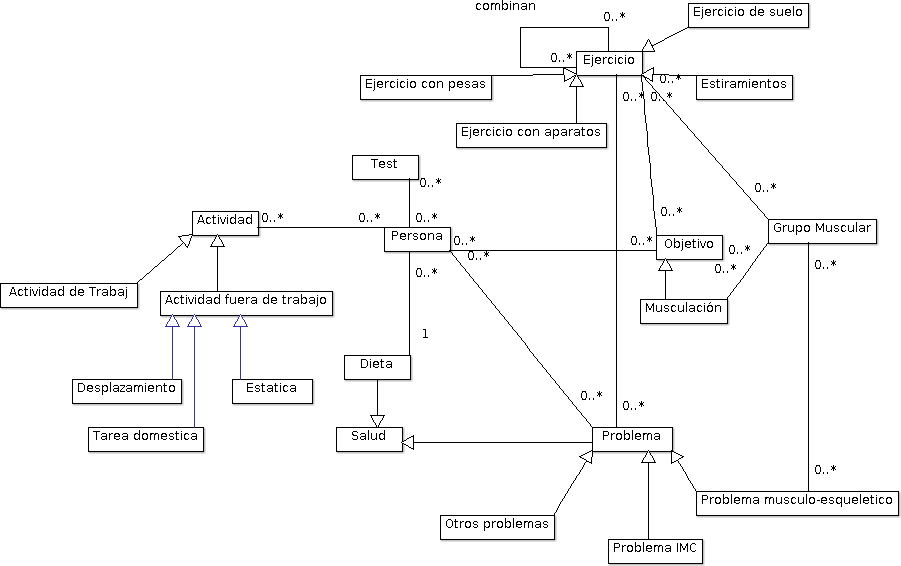
\includegraphics[width=\textwidth]{mainUML}
	\caption{Ontologia completa (Protege)}
\end{figure}

\pagebreak

Les classes que no estan especificades només hereten directament de la classe superior i no afegeixen cap camp. Només serveixen a nivell conceptual per facilitar la comprensió de la ontologia.

\subsubsection*{\underline{Exercici}}

És un dels conceptes principals de l'ontologia, ja que és el concepte que emmagatzema la informació necessària que permetrà saber si és una possible recomanació per a un determinat usuari. Conté els següents camps:

\begin{description}
	\item[Nom] de l'exercici
	\item[Calories cremades] El nombre de calories cremades per minut. 
	\item[Duració] màxima i mínima de l'exercici
	\item[Edat] màxima i mínima de l'exercici
	\item[Repeticions] màximes i mínimes de l'exercici
	\item[Exericis que combinen] Exercicis que està bé realitzar-los junt amb aquest exercici.
	\item[Grups musculars] Grups musculars que aquest exercici treballa.
	\item[Objectius] que l'exercici ajuda a assolir
	\item[Problemes alleujerats] Problemes associats a l'exercici que aquest ajuda a eliminar
	\item[Problemes contraindicats] Problemes pels quals realitzar l'exercici és perjudicial
\end{description}

\subsubsection*{\underline{Activitat}}

Representa una activitat física o estàtica que l'usuari realitza fora del gimnàs.

\begin{description}
	\item[Nom] de l'activitat
	\item[Freqüència] amb la que es realitza l'activitat, pot ser:
	\begin{itemize}
		\item Diària
		\item Setmanal
		\item Mensual
	\end{itemize}
	\item[Grau activitat] nivell d'activitat física d'aquesta, quan més alt més activa és l'activitat i quant més baix més sedentària és.
	\item[Duració] temps en minuts que dura l'activitat
\end{description}

\subsubsection*{\underline{Persona}}

Representa tota la informació que es té de l'usuari

\begin{description}
	\item[Nom] de l'usuari
	\item[Altura] alçada de la persona en metres.
	\item[Pes] en kg de l'usuari
	\item[Edat] anys de l'usuari
	\item[IMC] Índex de Massa Corporal (calculat a partir del pes i l'altura)
	\item[Pressió Màxima] pressió sanguínia màxima
	\item[Pressió Mínima] pressió sanguínia mínima
	\item[Problemes físics] Llista de problemes associats a l'usuari
	\item[Tests] Llista amb tots els tests que s'han fet a l'usuari (pot no haver-n'hi cap).
	\item[Activitats] llista amb totes les activitats que l'usuari realitza
	\item[Objectius] Llista amb tots els objectius que l'usuari ha seleccionat. 
\end{description}

\subsubsection*{\underline{Programa}}

Representa la solució final on hi ha tots els exercicis associats a cada dia

\begin{description}
	\item[Dilluns, Dimarts, Dimecres, Dijous, Divendres, Dissabte i Diumenge] Per cada camp hi ha els exercicis associats a cada dia que se li recomanen a l'usuari
	\item[Temps diari disponible] Llista de mida 7 (una setmana) on l'usuari pot posar el temps del que disposa cada dia de la setmana.
\end{description}

\subsubsection*{\underline{Test}}

Representa tota la informació que es pot obtenir d'un usuari a l'hora de realitzar un test.

\begin{description}
	\item[Nom] del test
	\item[PPM] Pulsacions per Minut de l'usuari just a l'acabar el test
	\item[Cansanci] relatiu just al finalitzar l'exercici (és un valor subjectiu) pot tenir els següents valors:
	\begin{itemize}
		\item Molt
		\item Poc
		\item Res
	\end{itemize}
	\item[Tirantor muscular] Quantitat de tirantor muscular que l'usuari nota al finalitzar l'exercici, pot tenir els següents valors:
	\begin{itemize}
		\item Molt
		\item Poc
		\item Res
	\end{itemize}
\end{description}

\subsubsection*{\underline{Salut}}

Aquesta classe només té l'atribut del nom ja que només serveix a la jerarquia per poder instanciar tot el que està relacionat amb la salut de l'usuari.  

\subsubsection*{\underline{Dieta}}

Representa la informació de la dieta de l'usuari, conté els següents camps:

\begin{description}
	\item[Nom] Nom de la dieta
	\item[Abús de sal] Nombre comprès entre 0 i 10 que representa l'abús de sal de l'usuari (0 gens, 10 molt).
	\item[Picar entre hores] Nombre comprès entre 0 i 10 que representa la quantitat de menjar que l'usuari pica entre hores (0 gens, 10 molt).
	\item[Consum de fruita] Nombre que representa la quantitat de peces de fruita de l'usuari durant una setmana.
	\item[Pastisseria] Nombre de peces de pastisseria que l'usuari menja durant una setmana.
\end{description}

\subsection{Mètode de resolució}

La classificació heurística es la metodologia de resolució de problemes de SBC que s'adapta al nostra cas, tenim un problema d'\textbf{anàlisis}. En aquest mètode l'expert escull una categoria d'un conjunt de solucions prèviament enumerades (la base de dades dels exercicis possibles a realitzar ofertes pel gimnàs). L'objectiu és obtenir i representar el coneixement necessari perquè l'associació de dades personals i peticions pugui realitzar-se i obtenir una recomanació possible com a solució.

Hem arribat a la conclusió de que tenim un problema d'anàlisis degut a que coneixem quin és el conjunt finit de solucions. Aquest conjunt està format per tots els exercicis que ofereix el gimnàs. En el nostre cas només és el subconjunt d'exercicis que hem escollit per instanciar, dins de tots els oferits pel gimnàs.

La classificació heurística es divideix teòricament en tres etapes (abstracció, associació heurística i refinament). Aquestes etapes encaixen el procés de resolució adquirit de l'expert. Així doncs, a continuació es detalla l'esquema de raonament de cada subproblema identificat a la conceptualització.

\subsubsection{Abstracció de dades}

Per un costat partim d'unes característiques del problema que són característiques que defineixen els usuaris ja sigui explícitament o implícitament, posant explícitament si desitgen que aquesta característica sigui un objectiu, un problema o una activitat a realitzar. 

També tenim la informació de l'estat físic de l'usuari a partir dels tests que aquest hagi pogut realitzar i que en el nostre cas s'haurà d'instanciar demanant-li a l'usuari que realitzi el test.

Si referenciem aquestes etapes des del nostre codi en CLIPS, el mòdul que pertany a aquesta fase és \verb|preguntas-persona|

\subsubsection{Associació heurística}

Un cop hem abstret la informació, és a dir, passar del \emph{Problema Concret} al \emph{Problema Abstracte}, llavors passarem a la següent fase en la que volem passar del \emph{Problema Abstracte} a la \emph{Solució Abstracta}. Aquesta fase la dividirem en dos parts:

En primer lloc hem de fer la inferència de les característiques que tenen els Exercicis que formen part del conjunt de la solució.

En segon lloc hem de fer la inferència de l'estat físic, és a dir, hem d'inferir de la mateixa manera que abans les característiques físiques que té l'usuari, però és important que no només tinguem en compte les característiques dels tests sinó que hem d'utilitzar el sentit comú per inferir les característiques que estan expressades implícitament.

Si ens centrem en referència al nostre codi de CLIPS, els mòduls que pertanyen a aquesta fase són: \verb|generar-solucion| on s'infereix el valor de l'estat físic de l'usuari.

\subsubsection{Refinament}

Un cop realitzades les dues fases anteriors, tan sols queda la última fase. Aquesta fase la dividirem en tres parts:

En primer lloc ens centrarem en descartar totes aquelles recomanacions on s'abstrau de l'usuari que no eren vàlides. Amb això ens assegurem que ninguna recomanació conté un subconjunt de solucions no vàlides.

En segon lloc, ens centrem en avaluar aquelles recomanacions on una determinada característica de l'exercici donat pel gimnàs és igual a la característica que s'ha inferit de l'usuari a partir dels tests o bé s'ha obtingut de l'usuari. Pel que amb això podem obtenir una justificació de perquè la solució serà vàlida més endavant, i el grau de recomanació que serà el que ens ajudi més endavant a saber amb quina preferència han d'aparèixer.

En aquesta tercera fase ens centrem en la ordenació de les recomanacions. Tal i com hem esmentat al paràgraf anterior, utilitzarem el grau de recomanació de manera que ens permeti saber en quin ordre hem d'oferir a l'usuari el conjunt solució d'exercicis, junt a una justificació.

Si ens centrem en referència al nostre codi de CLIPS, el mòdul que pertany a aquesta fase és \verb|generar-solució|.

\section{Implementació}

En aquesta fase ja tenim l'ontologia més adequada per representar el coneixement. També coneixem el mètode de resolució i els processos de raonament. Ara implementarem l'ontologia i encaixarem la descomposició de subproblemes amb la metodologia de classificació heurística. Tot això utilitzant el llenguatge CLIPS.

\subsection{Construcció de l'ontologia}

La representació final de l'ontologia la hem generat amb Protégé (\verb|"CouchPotato.pprj"|) i a més a més, al codi en CLIPS hem utilitzat 3 \verb|deftemplates| pels Exercicis, els temps i les puntuacions. Donat que hi ha una jerarqui a la classe 

\end{document}